\section{Produktudformning \label{sec:produktudformning}}
    \subsection{Lectio rework}
        \subsubsection{Overordnet}
           Lectio-applikationen er skrevet i et populært framework, Next.js, som er en overbygninng på React-biblioteket til node.js, der tillader at man kan køre javascript på en server i stedet for i Chrome V8-motoren, som kun tillader at man køre javascript clientsided fremfor serversided.

            React er et library for user interfaces, der tillader UI-komponenter, der i sammenspil med HTML, udgør en brugeroverflade. HTML står for >>HyperText Markup Language<<, der er standard markupsproget til alle hjemmesider--alt indhold, der serveres på internettet. Et markupsprog, fx. \LaTeX, som dette dokument er skrevet i, i modsætning til programmeringssprog, anvendes til at overlevere informationer til mennesker--programmeringssprog anvendes til at give instrukser til computere.

           Selve renovering er rent faktisk en renovering i den forstand, 
           at den reelle hjemmeside er blevet forbedret eller fornyet, 
           men derimod er den blevet genopygget fra bunden af dog med henblik på at bevare den samme funktionalitet. 
           Af den grund er det en mere korrekt betegnelse at kalde det et >>rework<<.
        \subsubsection{Kodegennemgang}
        Forneden er en komplet gennemgang af koden til Lectio-reworket.       

        En filstruktur behøver æstetisk, letoverskuelig og forståelig både i menneske- og computertermer.
        Således er der både de prædefinerede valg og de mere artistiske valg. 

        Et Next.js-projekt (v.14) benytter deres nyligt lancerede app router-filstruktursystem, således skal filer struktures på følgende vis: man har >>Top-level files<<, der bruges til applikationkonfiguration, administration af filafhængigheder m.m.\cite{projstruct}
        \begin{figure}[H]
        \dirtree{%
            .1 /.
            .2 {\color{blue}{app}}.
            .2 jsconfig.json.
            .2 LICENSE.
            .2 next.config.js.
            .2 {\color{blue}{node\_modules}}.
            .2 package.json.
            .2 package-lock.json.
            .2 postcss.config.js.
            .2 {\color{blue}{public}}.
            .2 REDME.md.
            .2 tailwind.config.js.
           }
        \caption{Top-level filstrukturen for lectio-reworket. Mapperne er farvet blåt}
        \label{fig:tlprojstruct}
        \end{figure}

        Forneden gennemgås top-level filerne og mapperne efter hensyn til forståelsen, der fremgår af figur (\ref{fig:tlprojstruct})

        \paragraph{next.config.js} er en konfigurationsfil for Next.js, der tillader, at man konfigurer sprogets funktionalitet. 
        
        \paragraph{LICENSE-filen} er en fil, der indeholder projektets licens og brugsrettigheder, og da vores er et open source-projekt (open source vil sige, at alle kan tilgå det "gratis"), så bruges MIT-licensen, der tillader al brug af materialet til alle formål af alle individer. 
        
        \paragraph{jsconfig.json} er en projektafhængighed for javascriptsproget, og den indeholder kompileringsvariabler, få. 

        \paragraph{tailwind.config.js. \label{par:tailwind}} er en konfigurationsfil, der konfigurer CSS. CSS er et understøttende design systemssprog til HTML, så alt der har med design at gøre, dvs. tekststørrelser, farver mv. "styles" i CSS. I Lectio.v2-applikation anvendes Tailwind-CSS, et framework til CSS, til at style dette; det er lettere overskueligt, hurtigere og standardiseret. Se forneden kode og rendering\ref{fig:modulbrikfostaaelse}:
        \begin{figure}[H]
            \begin{lstlisting}[language=HTML]
<div className="bg-[#9CCEFF] 
    border-l-[10px] 
    border-l-[#1E90FF] 
    p-4 
    rounded-lg 
    max-w-[275px] 
    max-h-[88px] 
    flex 
    justify-between 
    cursor-pointer 
    hover:opacity-80 
    group">

<div className="flex flex-col text-[#0D3F70] justify-center">
    <span className="font-bold text-xl">S 1x { args.subject }</span>
    <span>{ args.teacher }</span>
    <span>{ args.room }</span>
</div>    
            \end{lstlisting}
            \begin{center}
            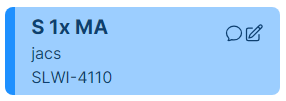
\includegraphics{assets/moduleElement.png}
            \end{center}
            \caption{Viser en modulbrik m. tilhørende CSS-kode (notér at dette ikke er den komplette kode [tjek bilag \ref{appendix:modulbrikkode}] til brikken, dog godt nok for at illustrere vores pointe) \label{fig:modulbrikfostaaelse}}
        \end{figure}
        \paragraph{app-mappen overordnet \label{pgh:app-ov}} indeholder reworkets reelle koder, i modsætning til de andre filer, der primært konfigurer koden og den gør kørbar. 
        Neden for ses hvordan vi har struktureret app-mappen. 
        \begin{figure}[H]
            \dirtree{%
                .1 app.
                .2 page.jsx.
                .2 layout.jsx.  
                .2 {\color{blue}{dashboard}}.
                .3 layout.jsx.
                .3 page.jsx.
                .2 {\color{blue}{lokaler}}.
                .3 page.jsx.
                .2 {\color{blue}{skema}}.
                .3 page.jsx.
                .3 skema.json.
                .3 {\color{blue}{[slug]}}.
                .2 {\color{blue}{ui}}.
                .3 {\color{blue}{dashboard}}.
                .3 {\color{blue}{navbar}}.
                .3 {\color{blue}{skema}}.
                .3 globals.css.
               }
            \caption{Filstrukturen for app mappen. Mapperne er farvet blåt}
            \label{fig:app-mappen}
            \end{figure}
        I Next.js, er alle mapper i /app-mappen, det er et subdomain, når det indeholder en >>page.jsx<<-fil. Men hvad er et subdomain? Før vi kan forstå det, skal vi se på, hvad er en URL? URL står for 
        Uniform Resource Locater. En URL er struktureret med først en protokol, som for web ressourcer er enten HTTP (Hypertext Transfer Protocol) eller HTTPS (HTTP Secure). Andre protokoller inkludere f.eks. FTP som er en >>File Transfer Protocol<<  
        efter protokollen kommer domænenavnet. Domænenavnet referer til en ip-adresse.  Det vil sige, at når man søger efter et domænenavn, søger man i en DNS-server (Domain Name System) og finder den tilknyttede ip-adresse,
        som sender den data, som hjememsiden består af til browseren. Efterfølgende kan der være subdomains der er alt efter domainenavnet plus et /.

        \begin{figure}[H]
        \begin{mdframed}
        \begin{equation*}
        \stackrel{\text{Internetprotokol}}{\overline{\text{https}}}:// \stackrel{\text{domænenavn}}{\overline{\text{noget.dk}}} / \stackrel{\text{subdomæne}}{\overline{\text{nogetandet}}}
        \end{equation*}
        \begin{center}
            Uniform Ressource Locater
        \end{center}
        \end{mdframed}
        \caption{Viser opbygningen af en URL}
        \end{figure}
        \newpage
        
        \paragraph{package.json} indeholder modulafhængigheder, der er hentet via NPM (Node package manager), der udnytter node.js. Forneden er et udsnit fra dette, der viser >>dependencies<<:
        \begin{lstlisting}[language=Javascript]
"dependencies": {
    "@heroicons/react": "^2.0.18",
    "@vercel/postgres": "^0.5.1",
    "bcrypt": "^5.1.1",
    "current-week-number": "^1.0.7",
    "dotenv": "^16.3.1",
    "heroicons": "^2.0.18",
    "next": "14.0.3",
    "react": "^18",
    "react-dom": "^18",
    "react-draggable": "^4.4.6"
    }, 
        \end{lstlisting}

        Mod venstre kan man se navnet på NPM-pakken. Efter kolonnet til højre ses versionen af denne. Næsten alle dem, der fremgår, bliver udnyttet, dog er der få som blot er resultatet af skabelonbrug. Denne skabelon er tiltænkt til fremtidig brug, så den kan anvendes til flere formål. Skabelonen kan også tilgås via GitHub.

        Her er en kort gennemgang af nogle af pakkerne, der er hentet via NPM, som vi bruger, der tilføjer ekstra funktionalitet:
        \begin{itemize}
        \item heroicons - Anvendes forskellige steder i koden, hvor ikoner anvendes. Heroicons fungerer således, at ønskede ikoner kan importeres fra heroicon-bibliotektet, hvorefter de kan indsættes i web-applikationen
        \item current-week-number - Anvendes til at fremkalde det nuværende ugetal via en applikation programm. Det i vores tilfælde til at indsætte ugetallet i skemabrikken. 
        \end{itemize}

        \paragraph{app-mappen}
            Vi startede med at gennemgå overordnet app-mappen (\ref{pgh:app-ov}), her er en dybdegående genemgang. App-mappen består af subdomænemapper og en UI-mappe (user interface).
            
            UI-mappen består af komponenter, fx. navigationsbaren, der anvendes på diverse web pages. Heraf er nogle af disse komponenter konsekvente på alle webpagesne, hvorfor det ikke giver mening at genskrive dem i hvert subdomæne. Disse konsekvente komponenter har ophav i root-layout.jsx mappen.
        
            \subparagraph{Layout.jsx-filen}
            \begin{figure}[H]
                \dirtree{%
                    .1 app.
                    .2 page.jsx.
                    .2 {\color{red}{layout.jsx.}}.
                    .2 {\color{blue}{dashboard}}.
                    .2 {\color{blue}{lokaler}}.
                    .2 {\color{blue}{skema}}.
                   }
                \caption{Filstrukturen for app mappen. Mapperne er farvet blåt}
                \begin{lstlisting}[language=Javascript]
import './ui/globals.css';
import { Inter } from 'next/font/google'
import Navbar_client from './ui/navbar/navbar-client'
import Navbar_server from './ui/navbar/navbar-server'

const inter = Inter({ subsets: ['latin'] })

export default function Layout({ children }) {

    return ( 
        <html lang="en">
            <body className={`${inter.className} antialiased flex justify-start`}>
                <Navbar_client>
                    <Navbar_server />
                </Navbar_client>
                {children}
            </body>
        </html> 
        );
}
                \end{lstlisting}
                \caption{Viser hvor layout.jsx (markeret rød) befinder sig i projektets filstruktur samt dens inhold \label{fig:layout}}
            \end{figure}
            Den importerer navbaren på klient- og serverside, hvorefter denne renderes, hvilket resulterer i, at den ikke behøves genrenderes hele websittets livscyklus.

            Måden, hvorpå navbaren forbliver det samme sted på div. webpages, er ved, at layout-filen agerer en overordnet skabelon, hvorefter subdomænernes og forsidens pagefils kode tilføjes under pladsholderen {children}.
            Se figur (\ref{fig:layoutforståelse}) nedenfor for forståelse.

            \begin{figure}[H]
                \centering
                \fbox{\resizebox{\columnwidth}{!}{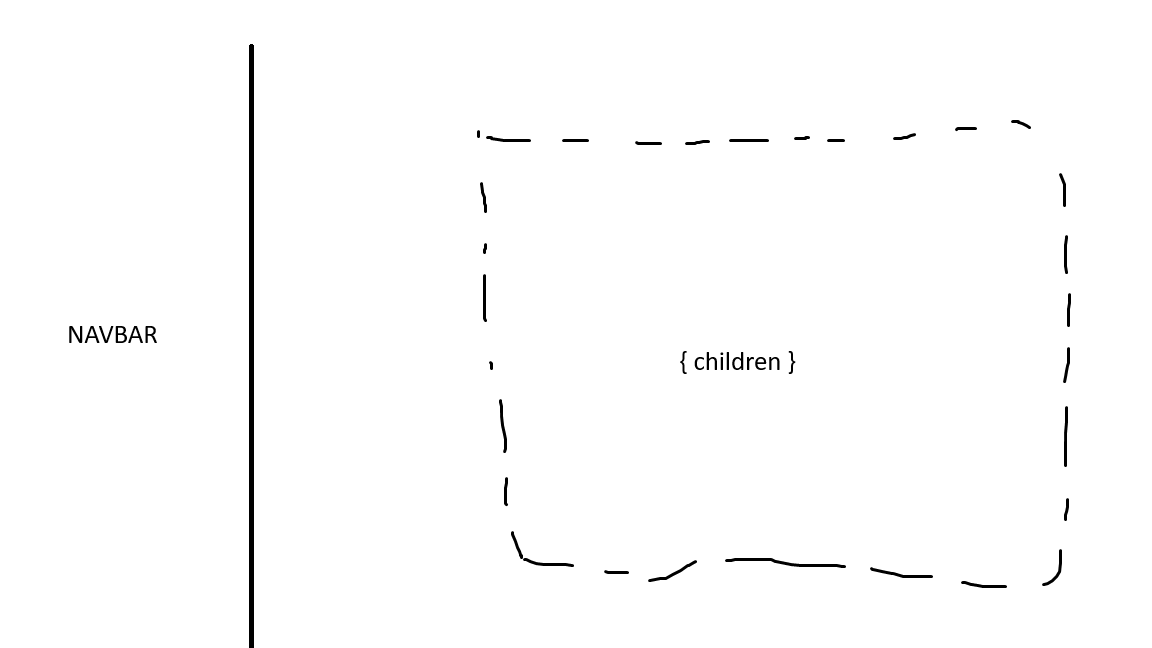
\includegraphics{assets/layout.png}}}
                \caption{Viser, hvordan layoutfilen påvirker webpagesnes rendering. \label{fig:layoutforståelse}}
            \end{figure}

            \subparagraph{page.jsx-filen}
            Page.jsx-filen er hjemmesidens forsidefil; det første forbruger møder. Page.jsx-filen indeholder tre primære HTML-sektioner (<div>), der på brugeroverfladen fremstår som kasser; som igen er stilet med CSS-tailwind (se paragraf \ref{par:tailwind}).

            \subparagraph{Skemakoden}
            Skemakoden er den del af Lectio-applikationen, vi har brugt mest tid på, da denne også dag-til-dag er vigtigst samt involverer databaseinfrastruktur. 
            
            Koden kan nedbrydes til dage, der kan nedbrydes til moduler. Dagene består et array (liste), hvor hvert et element i arrayet (listen) er et kodeobjekt, der indeholder modulsinformation, herunder faget, underviseren, lokation (lokale), noter, lektier samt metadata som synlighed (om folk skal se dig). Envidere indeholder det også et autogeneret ID, der anvendes til autogeneret web pages, der viser detajleret information om det individuelle modul.
            \begin{figure}[H]
                \begin{lstlisting}[language=Javascript]
// Monday
const scheduleMon = [
    { subject: 'MA', teacher: 'jacs', room: 'SLWI-4110', id: '1fxh', 
    visibility: 'show', note: 'Plan: Potensfunktioner, eksponentiel vaekst', homework: '03_opg_polynomier.ipynb' },
    
    { subject: 'MA', teacher: 'jacs', room: 'SLWI-4110', id: '123afa', 
    visibility: 'show', note: '', homework: '' },
    
    { subject: 'Fy', teacher: 'hnpo', room: 'SLWI-4110', id: 'qw123ac', 
    visibility: 'show', note: 'Ingen lektier. Vi ser paa hvad vi skal i timen. Forberedelse til SO2 i naeste uge. we  we jwnkjnkjn kjnkjnkjn ', homework: '' },
    
    { subject: 'Fy', teacher: 'hnpo', room: 'SLWI-4110', id: 'xcv12', 
    visibility: 'show', note: '', homework: '' },
    
    { subject: 'sa', teacher: 'mmje', room: 'SLWI-4110', id: 'sdvf23', 
    visibility: 'show', note: 'Det senmoderne samfunds kendetegn ', homework: '' },
    
    { subject: 'So', teacher: 'kibo', room: 'SLWI-4110', id: 'sdf123', 
    visibility: 'show', note: '', homework: 'Hold 'o'je med, hvordan du tager noter i de forskellige fag.' },
    
    { subject: '', teacher: '', room: '', id: 'sdv135', visibility: 'hide', note: '', homework: '' },
];
                \end{lstlisting}
                \caption{Viser et eksempel koden, der skal til for en dag. \label{fig:dataeksempel}}
            \end{figure}

        Alle dagene har et tilsvarende array med objekter. Selve skemaet er en kodetabel, der består af rækker (tablerowelement). SkemaModule-komponentet tager imod argumenter, hvilke hentes fra den tidligere sete kode. 
        \begin{figure}[H]
        \begin{lstlisting}[language=Javascript]
<td><SkemaModule subject={scheduleMon[0].subject}
<td><SkemaModule subject={scheduleTue[0].subject}
<td><SkemaModule subject={scheduleWed[0].subject}
<td><SkemaModule subject={scheduleThu[0].subject}
<td><SkemaModule subject={scheduleFri[0].subject}
        \end{lstlisting}
        \caption{Viser at >>SkemaModule<<-komponentet tager første (nulte i kode) objekt i schedule<dag>'s kodeproperty (properties er en værdi, der tilhører et objekt). SkemaModule modtager langt flere properties fra de respektive objekter, fx lærer, fag osv.; dett er et udsnit--se appendiks \ref{appendix:SkemaModule} for resterende kode.}
        \end{figure}
       
        \subparagraph{SkemaModule.jsx}
        SkemaModule.jsx-filen indeholder det komponent, der referers tidligere >>SkemaModule<<, heri bliver argumenterne indsat i HTML-kode, hvor der et script, der tjekker om args.note er tom, altså om der er lektionnoter, for det pågældende modul--hvis denne ikke er tom (altså \textit{indeholder}), viser den et ikon, og det samme sker med args.homework, således at "lektieikonet" vises. Ligeledes dukker "tooltips" også op, når brugerens mus er over et modulelement, dog udover at der tjekkes om argumenterne/propertiesne er tomme, importeres værdien og renderes i selve tooltippet. Se figur for forståelse:

        \begin{figure}[H]
        \centering
        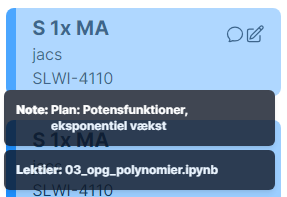
\includegraphics{assets/moduleElement2.png}
        \caption{Viser et modul, hvis args.note og args.homework-argumenter/properties ikke er tomme samt har værdier; ligeledes de respektive tooltips og ikoner.}
        \end{figure}
        
        \subparagraph{Datohåndteringssystem}
        Datahåndteringssystemet fungerer på den måde, at der op i toppen defineres et array med datoer, dette er datoerne, der fremgår på vores skemaeksempel; hvis softwaren skulle distribueres ville disse blive indhentet via en API (Application programming interface), således datoerne bliver dynamisk opdateret.

        Forneden fra linje 4-10 indhentes dagens dato, hvorefter denne anvendes til at skrive dags dato. Herefter laves en konstant, der tager variablerne >>date<< og >>month<<, disse anvendes senere ned til at blive sammenlignet med >>Current 
        \begin{lstlisting}[language=Javascript]
const weekNumbers = ["29/4", "30/4", "1/5", "2/5", "3/5"];


const today = new Date();
const month = today.getMonth()+1;
const year = today.getFullYear();
const date = today.getDate();
const currentDate = month + "/" + date + "/" + year;

const currentFormattedDate = month + "-" + date + "-" + year; 

const weekDate = date + "/" + month;

var currentWeekNumber = require('current-week-number');

// Her er en masse kode imellem se appendiks F

{ (() => {
    if (weekNumbers[0] == weekDate) {
        return (
            <span className="px-10 p-4 rounded-xl bg-[#1E90FF] text-white font-normal">Mandag <strong>{ weekNumbers[0] }</strong></span> 
        );
    } else {
        return (
            <span className="px-10 p-4 rounded-xl bg-slate-200 font-normal">Mandag <strong>{ weekNumbers[0] }</strong></span>
        );
    }

})()}
        \end{lstlisting}
    Herefter tjekker koden om den pågældende ugedag er lig med dags dato, hvorefter dennes respektive UI-element i så fald gøres blåt for at indikere til brugeren, at denne dad er dags dato.
    
    \subparagraph{Dynamic Routes (slugs)}
    Dynamic routes er "ruter" til data, hvis specifikke lokation vi ikke kender i forvejen (generer subdomæner dynamisk ud fra input). Dynamic routes anvendes i dette tilfælde til automatisk generation af sider med et respektivt moduls deltajeret information og oversigter, herunder vehæftelser. 
    Denne genereres ved, at der i skemasubdomænet eksisterer et subsubdomæne med square brackets herom [], hvilket fortæller dokumentet er der er tale om et dynamisk sub(sub)domæne, hvori der ligger en page.jsx-fil tilsvarende til dem, vi har gennemgået tidligere, dog er denne 100\% dynamisk, og der specificeres, hvordan information skal formateres, men selve informationen / indholdet hentes via et API fra en anden webserver / serverdatabase. Datasvaret, vi ville få, er samme type som vores skemakoder anvender (objekter), ergo næsten ens, da dette også er .JSON-format--se tidl. figur for dataeksempel \ref{fig:dataeksempel}. 
        \begin{figure}[H]
        \centering
        \resizebox{\columnwidth}{!}{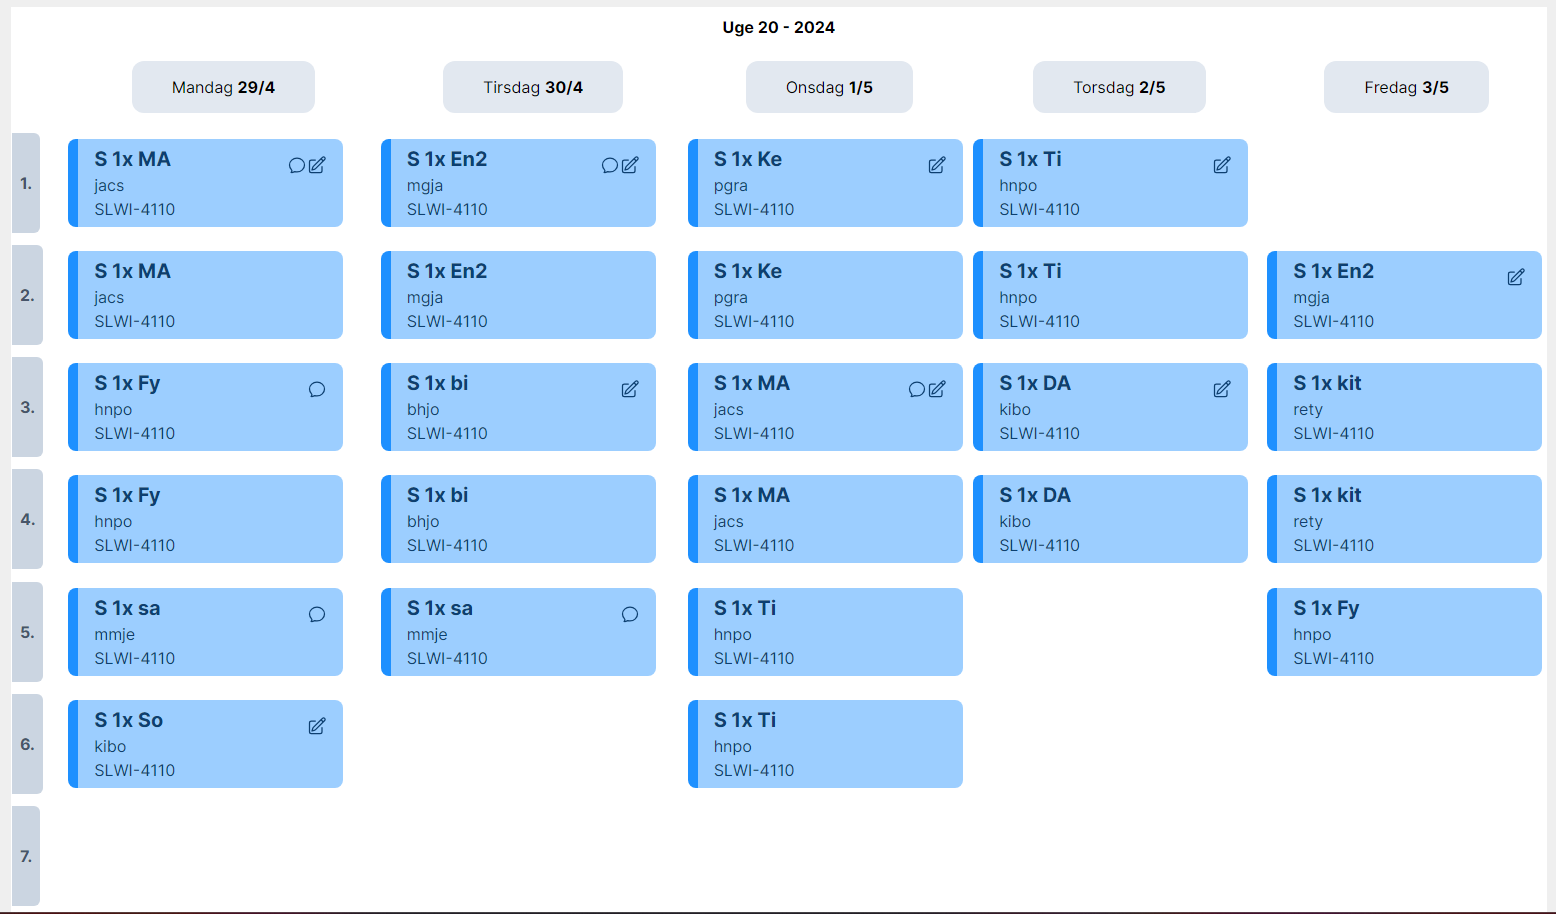
\includegraphics{assets/skemaElement.png}}
        \caption{Viser skemaet.}
        \end{figure}
\subsection{Bookingsystem}
    Vi har valgt at fjerne bookingsystems-delen for dette produkt; dog er den skidegod ide, og det var blevet en del af produktet. Det er af rent pragmatiske årsager, at vi vælger ikke at udvikle systemet, det havde garanteret været sjovt. Skitserne over dette fremgår af appendiks \ref{appendix:arbejdsskitser}.

\subsection{RFID-System}
    \subsubsection{Overordnet}
    Som del af vores teknologiprojekt fandt vi frem til at vi kunne forbedre studiemiljøet ved at implementere døre på skolen der benytter sig af RFID (Radio-frequency identification). 
    Og udlevere studiekort til elever som de kan benytte sig af til f.eks. at åbne bookede lokaler eller til hurtigere at tage fravær,
    og i tilfælde af brand ville der også være mulighed for at låse alle døre op til potentielle flugtveje. disse er alle ting som er med til at modernisere IT-Infrastrukturen på skolen, 
    og derved forbedre studiemiljøet for elever.

    \subsubsection{Konstruktion}
    Da vi gik i gang med at planlægge konstruktionen af produktet kom vi ret hurtigt frem til at det ikke ville være en mulighed at bygge en dør med scanneren på, vi besluttede derfor at,
    vi ville konstruere en primitiv prototype i stedet for, som en form for repræsentation af hvad det rigtige produkts egenskaber ville være. vi har dog lavet alle overvejelserne til det rigtige produkt.
    den prototype er placeret i en gammel kasse vi havde, da det stadigvæk fint repræsenterer funktionaliteten af produktet, inde i kassen er der et stort breadboard, esp-wroom32 (devkitC variant),
    en lille powersupply der bruger et lithium-ion batteri, 2 led'er, og en RFID-RC522 scanner. disse komponenter er alt der der skal til for at få selve hardware delen til at virke. 
    for at korrekt sammensætte disse komponenter fulgte vi dokumentationen for RFID-RC522 scanneren som vi fandt online, efterfølgende tilføjede vi de ting der skulle til for at få prototypen til at repræsentere
    det vores produkt skulle kunne. opsætningen af esp32'eren var lidt udfordrene men fandt heldigvis nogen guides der beskrev nogle hovedpunkterne i forhold til opsætning.
    
    men før vi gik i gang med at bygge selve kassen havde vi lavet et diagram i EasyEda der viste hvordan at prototypen ville komme til at se ud.'
    
    \begin{figure}[H]
        \centering
        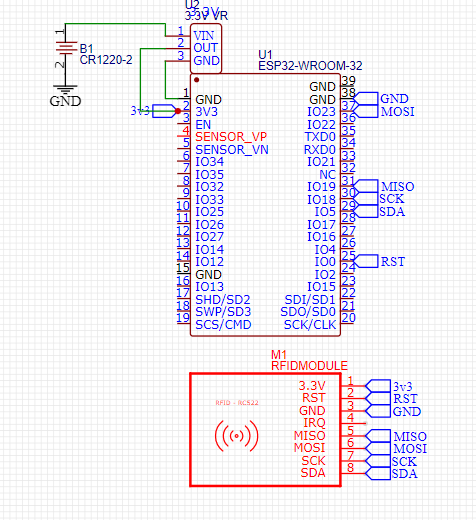
\includegraphics{assets/internalDiagram.png}
        \caption{Internt Diagram RFID-System}
    \end{figure}
    
    som det kan ses på skitsen har vi planlagt hvordan de forskellige komponenter skulle kobles sammen før vi gik i gang med at bestille delene hjem til produktet, selve udformningen og konstruktionen af produktet tog ikke særligt lang tid.
    den mest tidskrævende del af processen var at regne ud hvordan vi ville lave dør systemet, i starten overvejede vi at lave den som en knap på en app man kunne bruge til at låse døren op,
    men kom frem til at det var nemmere både produkt mæssigt men også for brugeren hvis døren benyttede sig af RFID da du der både har mulighed for at bruge en app på din Telefon, og et kort/chip til at låse døren op.


    \subsubsection{Kodegennemgang}

    Programmeringen af Esp'en viste sig også at være lidt af en udfordring da efter vi havde koblet alting sammen, kunne vi ikke få lov til at uploade kode til den. dette viste sig at tage noget tid at løse,
    så lad og gå igennem min process med at løse det.

    \begin{enumerate}    
        \item Vores første problem var at Arduino IDE ikke havde muligheden for at vælge den ESP32 som vi brugte, vi ledte en del tid efter nogen der havde en løsning, og kom frem til at det er fordi at den ESP32 vi bruger,
            ikke har sin egen kategori når du vælger hvilket board (Arduinoen) du bruger, men at den går ind under "Dev Module" kategorien.

        \item Det andet problem vi stødte på var at vi ikke kunne se den COM port (Communications/Serial Port) som min ESP32 kørte over, dette skyldes at vi manglede en driver der hedder "CP210x Universal Windows Driver",
            den gør det muligt for min computer at åbne de COM porte vi skulle benytte, og da den driver ikke var på min computer kunne vi ikke koble min ESP32 op.
        
        \item Det sidste problem vi stødte på var at selvom vi var koblet op til min ESP32 blev den ved med at give os fejlkoden "Wrong boot mode detected, device needs to be in download mode", dette forvirrede os lidt,
            da vi ikke var sikker på hvordan vi havde mulighed for at ændre hvilket boot mode min ESP32 var i. Dette problem var dog relativt nemt at løse da det viste sig at man skulle holde boot knappen på Esp'en nede,
            når man uploadede ting til den.
    \end{enumerate} 
        
        Efter vi havde overkommet de initiale udfordringer med Programmeringen, gik det faktisk overraskende nemt, det lykkedes os at finde et "Library" der havde eksempel kode der mindede meget om det vi havde brug for,
        til at få min scanner til at virke. \newline
        Se Bibliografi for kilder brugt til udvikling af ovenstående, \cite{ardDrive}, \cite{ardrfid}, \cite{ardProg}
